\newcommand{\files}[1]{
    \hfill\,
    \mbox{
        $\hookrightarrow$
        \texttt{#1}
    }
}

\section{Mikrofone}
\label{sec:1}
In dieser Hausaufgabe werden die akustischen Eigenschaften einer Auswahl an Mikrofonen (siehe Tabelle \ref{tab:mics}) analysiert und miteinander verglichen.
Als Grundlage stehen die Frequenzgangsdaten der Schalldruckpegel aus verschieden Einfallsrichtungen zur Verfügung.

\def\arraystretch{1.3}
\begin{table}[h]
    \centering
    \caption{Auswahl der Mikrofone}
    \label{tab:mics}
    \begin{tabular}{l l l l l}
        Hersteller & Typ & Akustische Arbeitsweise & Richtcharakteristik & Einfallsrichtung \\
        \hline
        Shure & \texttt{SM58} & Druckgradienten- und Schnelleempfänger & Niere & 0°, 90°, 180° \\
        Neumann & \texttt{KM120} & Druckgradienten- und Auslenkungsempfänger & Acht & 0°, 90°, 180° \\
        Neumann & \texttt{KM184} & Druckgradienten- und Auslenkungsempfänger & Niere & 0°, 5°, ..., 180°
    \end{tabular}
\end{table}


\subsection{\texttt{K120} und \texttt{SM58} bei Frontalschalleinfall}
\label{subsec:a}
Aus den zur Verfügung gestellten "`\texttt{*\_0.txt}"' Dateien werden die für die Abbildung \ref{fig:freq_0} benötigten Informationen bei frontalem Schalleinfall extrahiert.
Dabei wird jeweils ein Offset ermittelt und angewandt, der den Schalldruckpegel der eingelesenen Informationen bei 1000 Hz auf 0 dBV normiert.
Zur Weiterverarbeitung im Aufgabenteil \ref{subsec:c} werden die Offsets zwischengespeichert.
\files{main.m, ImportTarget.m}

\begin{figure}[bth]
    \centering
    \begin{subfigure}{.5\textwidth}
        \centering
        \caption{KM120}
        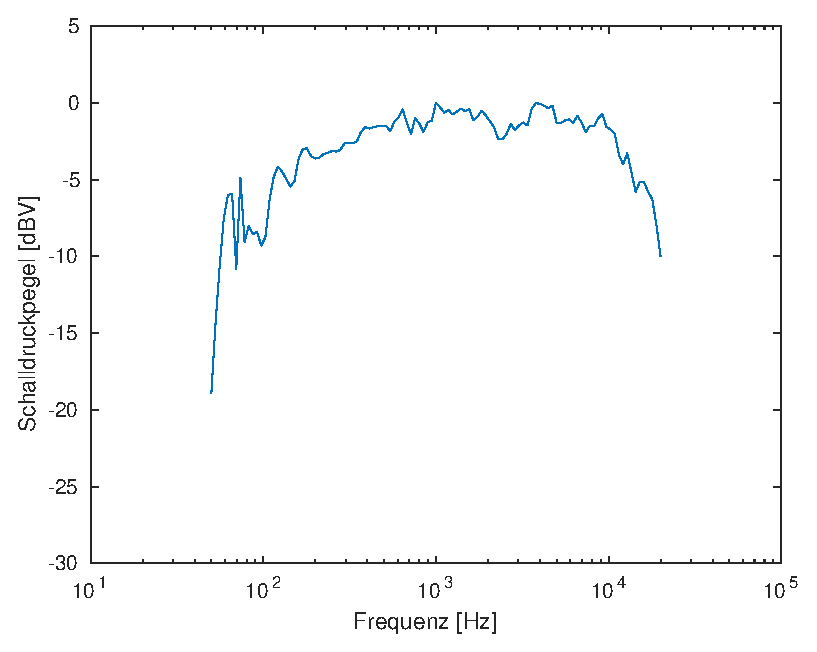
\includegraphics[width=0.95\linewidth]{Figures/km120_0}
    \end{subfigure}%
    \begin{subfigure}{.5\textwidth}
        \centering
        \caption{SM58}
        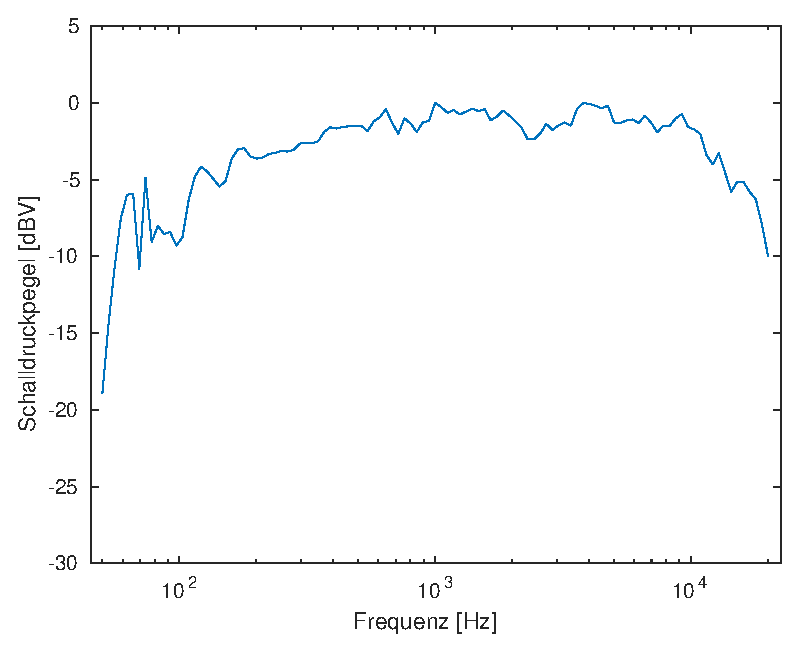
\includegraphics[width=0.95\linewidth]{Figures/sm58_0}
    \end{subfigure}
    \caption{Frequenzgänge der Mikrofone bei Frontalschalleinfall normiert auf 0 dBV bei 1000 Hz}
    \label{fig:freq_0}
\end{figure}

\subsection{Glättung der Frequenzgänge}
\label{subsec:b}
Für die Implementierung des gleitenden Mittelwerts verwenden wir Matlabs \texttt{MovMean()} Methode.
Das resultierende, geglättete Spektrum ist in Abbildung \ref{fig:freq_movmean} zu sehen. Das Verhältnis benachbarter Frequenzbins ist konstant und beträgt $f_{n+1}/f_{n} = 1.057$.
Die Implementierung des gleitenden Mittelwerts nehmen wir mit der filter() Methode aus Matlab vor.
Das resultierende geglättete Spektrum ist in Abbildung \ref{fig:freq_movmean} zu sehen. Das Verhältnis benachbarter Frequenzbins ist konstant und beträgt $f_{n+1}/f_{n} = 1.057$.
Die Frequenzauflösung der Spektren ist somit nicht linear, sondern abhängig von der Frequenz.
Zudem mittelt der gleitende Mittelwert konstant über drei Bins.
Das bedeutet, dass es sich um eine Glättung mit relativer Bandbreite handelt.
Allerdings ist es weder eine terzbreite noch eine oktavbreite Glättung.
In beiden Fällen müsste das Frequenzverhältnis benachbarter Bins größer sein.
Allgemein gilt: Eine Glättung mit relativer Bandbreite liefert eine gleichmäßigere Kurve in logarithmischer Darstellung der Frequenzachse des Spektrums, als eine Glättung mit konstanter Bandbreite.
Letztere liefert wiederum eine gleichmäßig geglättete Kurve für eine Darstellung mit linearer Frequenzachse.

\begin{figure}[bth]
    \centering
    \begin{subfigure}{.5\textwidth}
        \centering
        \caption{KM120}
        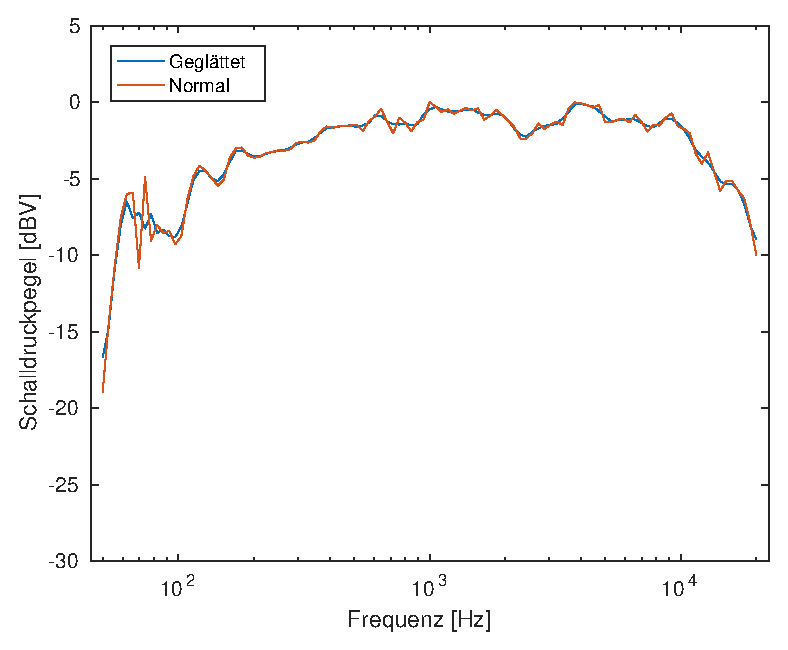
\includegraphics[width=0.95\linewidth]{Figures/km120_0_movmean}
    \end{subfigure}%
    \begin{subfigure}{.5\textwidth}
        \centering
        \caption{SM58}
        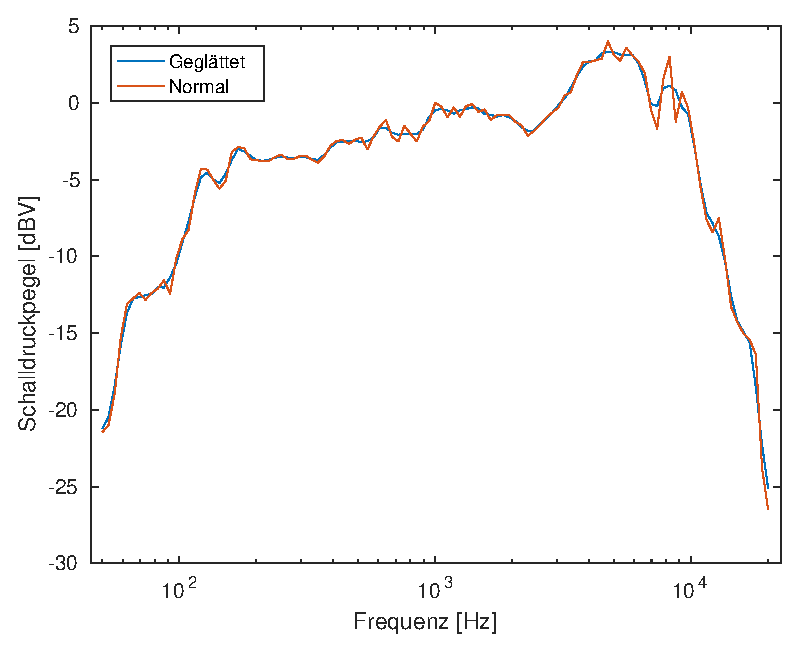
\includegraphics[width=0.95\linewidth]{Figures/sm58_0_movmean}
    \end{subfigure}
    \caption{Unterschied zwischen dem normalen und dem geglätteten Frequenzgang der Mikrofone bei frontalem Schalleinfall}
    \label{fig:freq_movmean}
\end{figure}
Wie erwartet führt die Glättung zu einer weicheren Kurve. 
Vergleichen wir unsere Darstellung der Frequenzgänge mit denen auf den Websites des Herstellers Neumann \footnote{\url{https://www.neumann.com/assets/diagrams/km100_diagrams.htm}} und des Herstellers Shure \footnote{\url{https://www.shure.de/produkte/mikrofone/sm58}} fällt auf, dass die Frequenzgänge auf den Websites  um einiges stärker geglättet sind.
\files{main.m, MovMean.m}

\subsection{\texttt{K120} und \texttt{SM58} für alle Einfallsrichtungen}
\label{subsec:c}
Die im Aufgabenteil \ref{subsec:a} extrahierten Informationen zum frontalen Schalleinfall werden nun um die beiden Einfallsrichtungen bei 90° und 180° erweitert.
In diesem Fall kommen die in Aufgabe \ref{subsec:a} zwischengespeicherten Offsets für die Normierung der Schalldruckpegel zum Einsatz, damit die Schalldruckpegel für alle Einfallswinkel den gleichen Referenzwert haben.
Die Frequenzen der neu extrahierten Informationen werden ebenfalls geglättet und sind gemeinsam mit dem geglätteten Frontalschalleinfall aus Aufgabenteil \ref{subsec:b} in Abbildung \ref{fig:freq_all} dargestellt.


\begin{figure}[bth]
    \centering
    \begin{subfigure}{.5\textwidth}
        \centering
        \caption{KM120}
        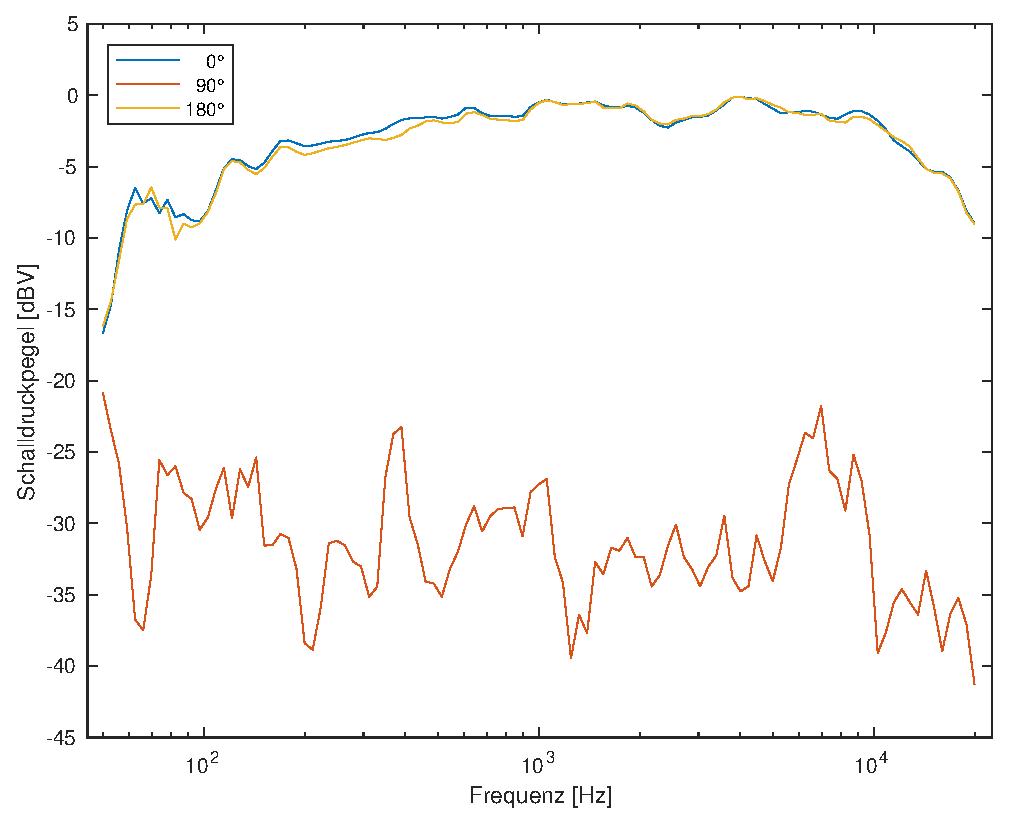
\includegraphics[width=0.95\linewidth]{Figures/km120_all}
        \label{fig:km_sm}
    \end{subfigure}%
    \begin{subfigure}{.5\textwidth}
        \centering
        \caption{SM58}
        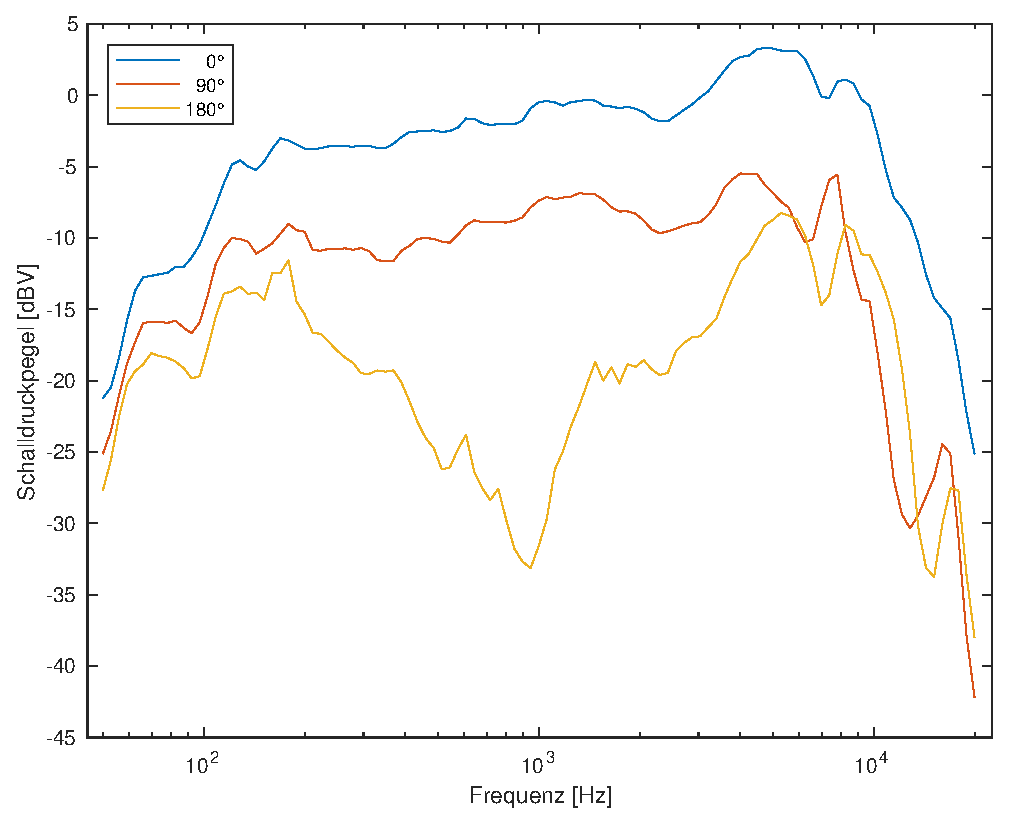
\includegraphics[width=0.95\linewidth]{Figures/sm58_all.eps}
    \end{subfigure}
    \caption{Geglättete Frequenzgänge aus drei verschiedenen Einfallsrichtungen}
    \label{fig:freq_all}
\end{figure}

Die 0° Frequenzgänge des Neumann und Shure Mikrofons unterscheiden sich insofern, dass die Empfindlichkeit des Shure Mikrofons bei hohen Frequenzen ansteigt und die des Neumann Mikrofons näherungsweise konstant bleibt (siehe Abbildung \ref{fig:km_sm})
Dies lässt sich mit der Tatsache erklären, dass beide Mikrofone Druckgradientenempfänger sind, was zunächst zu einer mit der Frequenz ansteigenden Empfindlichkeit führt.
Der Effekt wird beim Neumann Mikrofon allerdings kompensiert, da es sich um einen Auslenkungsempfänger handelt, bei dem die Empfindlichkeit mit der Frequenz abnimmt.
Beim Shure Mikrofon bleibt dieser Effekt aus, da Schnelleempfänger eine frequenzunabhägige Empfindlichkeit aufweisen.\\
Die Richtungsabhängigkeit der Frequenzgänge (siehe Abbildung \ref{fig:freq_all} stimmt mit den Richtcharakteristiken der beiden Mirkofone überein. 
Beim KM120 haben wir fast identische Frequenzgänge für die Einfallsrichtungen 0° und 180° und nur sehr geringe Empfindlichkeiten in 90° Richtung, passend zur Acht-Charakteristik.
Beim SM58 sinkt die Empfindlichkeit bei allen Frequenzen mit steigender Winkeldifferenz zur 0° Richtung, passend zur Nierencharakteristik.
Auffallend ist dabei, dass tiefe und hohe Frequenzen für die 180° Einfallsrichtung nicht so stark absinken, wie die mittleren Frequenzen.
Das starke Absinken entspricht dem Verhalten einer idealen Niere, bei hohen und tiefen Frequenzen gibt es also Abweichungen von der typischen Nierencharakteristik.  
\files{main.m, ImportOffset.m, MovMean.m}


\subsection{Richtcharakteristik des \texttt{KM184}}
\label{subsec:d}
Die frequenzabhängigen Richtcharakteristiken des Neumann KM184 sind in Abbildung \ref{fig:Polar_sep} zu sehen.
Die Richtcharakteristik liegt je nach Frequenz zwischen Breiter Niere und Niere. 
Die Richtcharakteristiken bei 125 Hz hat die Form einer Breiten Niere, die Charakteristiken zwischen 250 Hz und 8000 Hz sind nierenförmig und bei 16000 Hz erkennen wir eine Superniere.
Beim Vergleich mit den frequenzabhängigen Charakteristiken auf der Webseite \footnote{\url{https://www.neumann.com/assets/diagrams/s180_diagrams.htm}} des Herstellers Neumann können wir keine deutlichen Unterschiede erkennen.
\files{main.m}

\begin{figure}[bth]
    \centering
    \begin{subfigure}{.25\textwidth}
        \centering
        \caption{125 Hz}
        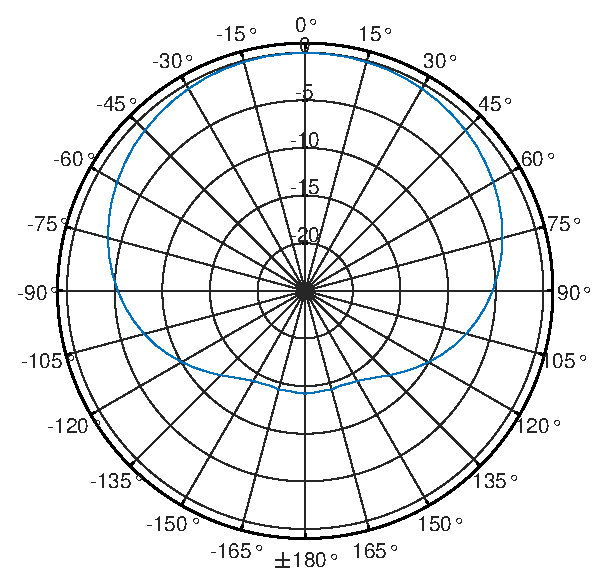
\includegraphics[width=\linewidth]{Figures/KM184_125Hz}
        \label{fig:Polar_125}
    \end{subfigure}%
    \begin{subfigure}{.25\textwidth}
        \centering
        \caption{250 Hz}
        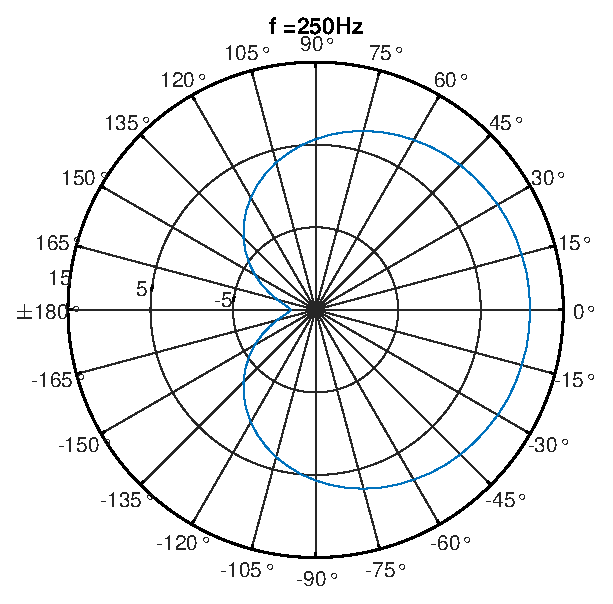
\includegraphics[width=\linewidth]{Figures/KM184_250Hz}
        \label{fig:Polar_250}
    \end{subfigure}%
    \begin{subfigure}{.25\textwidth}
        \centering
        \caption{500 Hz}
        \includegraphics[width=\linewidth]{Figures/KM184_500Hz}
        \label{fig:Polar_500}
    \end{subfigure}%
    \begin{subfigure}{.25\textwidth}
        \centering
        \caption{1000 Hz}
        \includegraphics[width=\linewidth]{Figures/KM184_1000Hz}
        \label{fig:Polar_1000}
    \end{subfigure}

    \begin{subfigure}{.25\textwidth}
        \centering
        \caption{2000 Hz}
        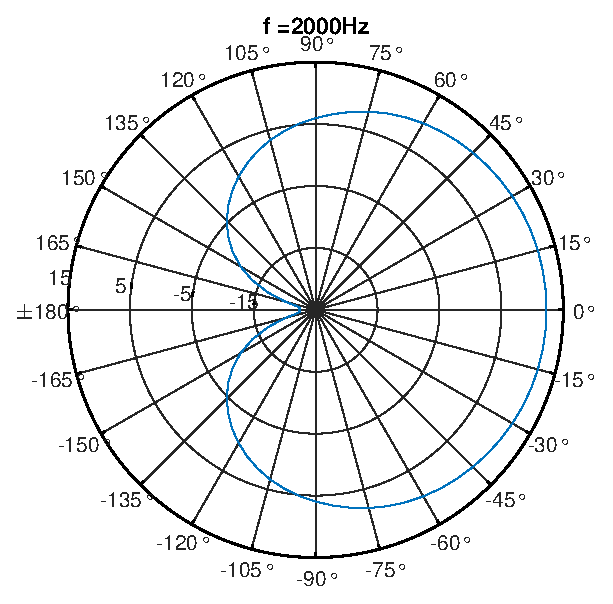
\includegraphics[width=\linewidth]{Figures/KM184_2000Hz}
        \label{fig:Polar_2000}
    \end{subfigure}%
    \begin{subfigure}{.25\textwidth}
        \centering
        \caption{4000 Hz}
        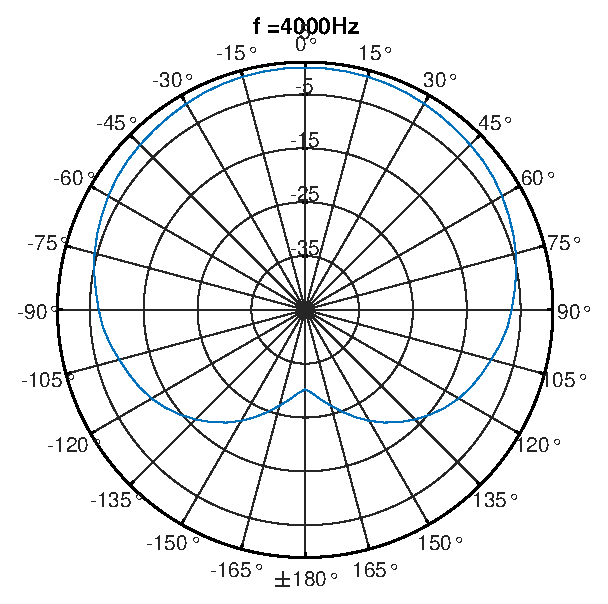
\includegraphics[width=\linewidth]{Figures/KM184_4000Hz}
        \label{fig:Polar_4000}
    \end{subfigure}%
    \begin{subfigure}{.25\textwidth}
        \centering
        \caption{8000 Hz}
        \includegraphics[width=\linewidth]{Figures/KM184_8000Hz}
        \label{fig:Polar_8000}
    \end{subfigure}%
    \begin{subfigure}{.25\textwidth}
        \centering
        \caption{16000 Hz}
        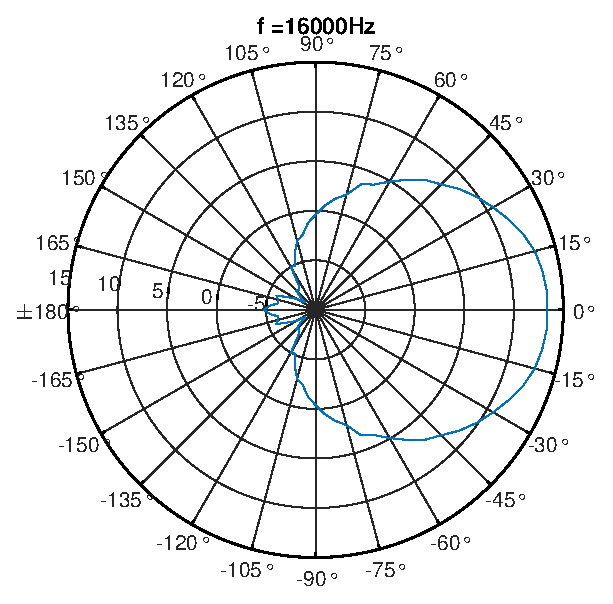
\includegraphics[width=\linewidth]{Figures/KM184_16000Hz}
        \label{fig:Polar_16000}
    \end{subfigure}
    \caption{Richtcharakteristik des \texttt{KM184} aufgeteilt in Frequenzen}
    \label{fig:Polar_sep}
\end{figure}


\subsection{Bündelungsgrad und Bündelungsmaß}
\label{subsec:e}
Der frequenzabhängige Bündelungsgrad des Neumann KM184 ist in Abbildung \ref{fig:buendel} dargestellt. 
Laut dem Handbuch der Audiotechnik \cite{Weinzierl08} hat eine Niere gemäß der Berechnung mithilfe der idealisierten Richtcharakteristik $A + B \mathrm{cos}(\theta)$ den Bündelungsgrad 3, eine Breite Niere den Bündelungsgrad 1,89 und eine Superniere den Bündelungsgrad 3,73.
Demnach nähert sich der mit der Frequenz moderat steigende Bündelungsgrad des KM184 zwischen 100 Hz und ca. 5000 Hz zunehmend dem einer Niere an.
Dann kommt es zu einem Einbruch zwischen ca. 6000 Hz und 10000 Hz, wo der Bündelungsgrad bis auf einen für eine breite Niere typischen Wert abfällt. 
Für höhere Frequenzen steigt $\gamma$ nochmal stark an und erreicht  Super- und Hypernierentypische Werte.
\files{main.m}

\begin{figure}[bth]
    \centering
    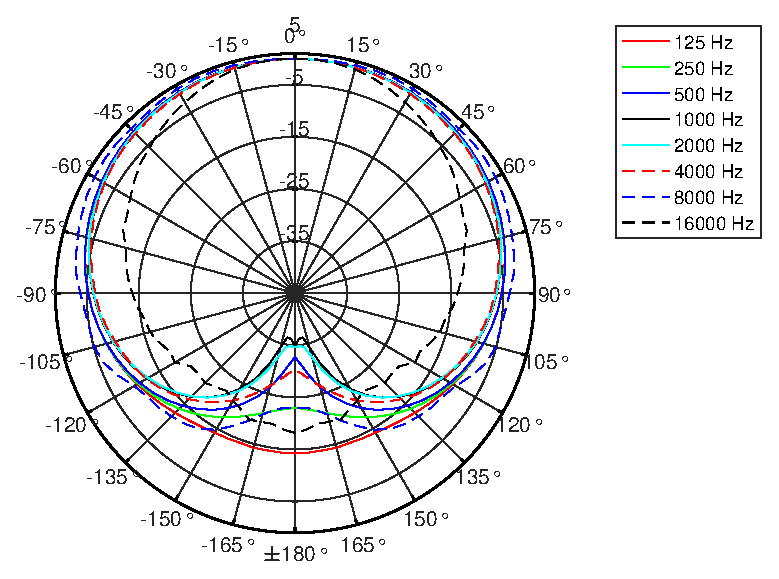
\includegraphics[width=\linewidth]{Figures/KM184_allfreqs}
    \caption{Alle Frequenzen}
    \label{fig:Polar_allfreqs}
    \caption{Zusammengefasste Richtcharakteristik des \texttt{KM184}}
\end{figure}

\subsection{Bündelungsgrad}
Der frequenzabhängige Bündelungsgrad des Neumann KM184 ist in Abbildung ??? dargestellt. 
Laut dem Handbuch der Audiotechnik \cite{Weinzierl08} hat eine Niere gemäß der Berechnung mithilfe der idealisierten Richtcharakteristik $A + B \mathrm{cos}(\theta)$ den Bündelungsgrad 3, eine breite Niere den Bündelungsgrad 1,89 und eine Superniere den Bündelungsgrad 3,73.
Demnach nähert sich der mit der Frequenz moderat steigende Bündelungsgrad des KM184 zwischen 100 Hz und ca. 5000 Hz zunehmend dem einer Niere an.
Dann kommt es zu einem Einbruch zwischen ca. 6000 Hz und 10000 Hz, wo der Bündelungsgrad bis auf einen für eine breite Niere typischen Wert abfällt. 
Für höhere Frequenzen steigt $\gamma$ nochmal stark an und erreicht  Super- und Hypernierentypische Werte.

\begin{figure}[H]
    \centering
    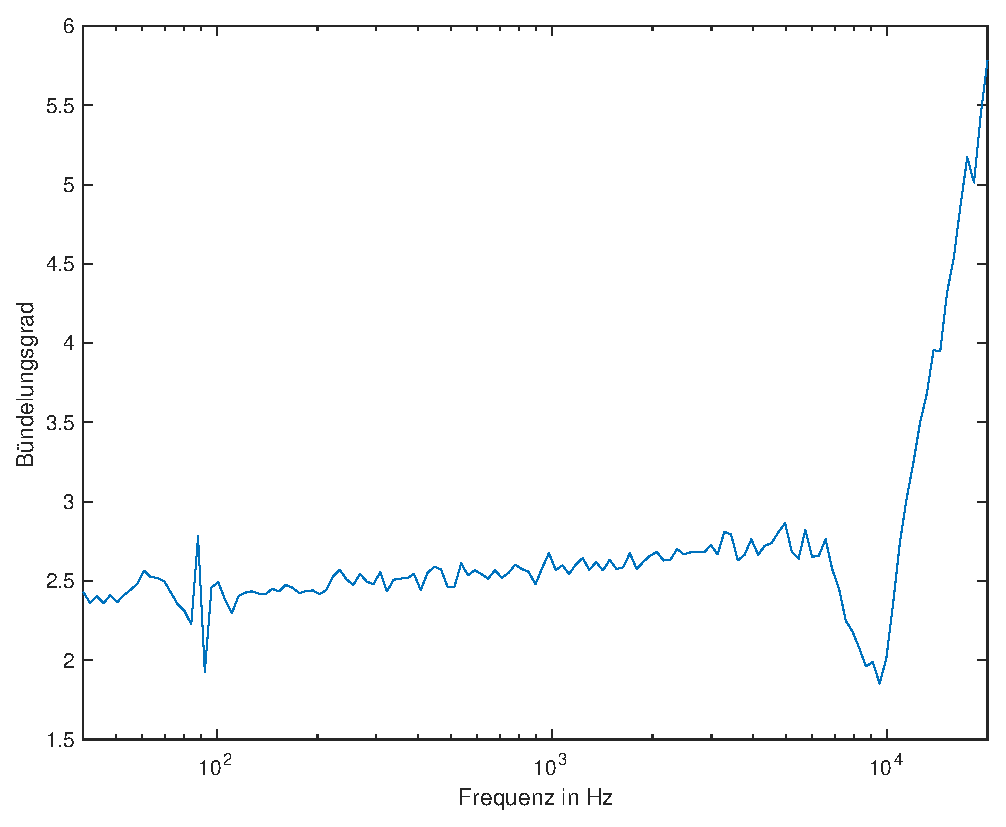
\includegraphics[width=0.8\linewidth]{Figures/Buendelungsgrad}
    \label{fig:buendel}
    \caption{Bündelungsgrad des Neumann KM184 in Abhängikeit der Frequenz}
\end{figure}






